\subsection{Question 1}

\begin{figure}[H]
  \centering
  \begin{tikzpicture}
    % Liste des places
    \draw (-9,0) node[below left = 2pt] {$O_7a$};
    \node[draw,circle,scale=2] (o7a) at (-9, 0) {};
    \draw (-7,0) node[above left = 2pt] {$O_7b$};
    \node[draw,circle,scale=2] (o7b) at (-7, 0) {};
    \draw (-5, -7) node[below right = 2pt] {$O_6b$};
    \node[draw,circle,scale=2] (o6b) at (-5, -7) {};
    \draw (-5,-9) node[above right = 2pt] {$O_6a$};
    \node[draw,circle,scale=2] (o6a) at (-5, -9) {};
    \draw (-5,-3) node[below right = 2pt] {$E_7$};
    \node[draw,circle,scale=2] (e7) at (-5, -3) {};
    \draw (-5,-1) node[below right = 2pt] {$E_1$};
    \node[draw,circle,scale=2] (e1) at (-5, -1) {};
    \draw (-5,7) node[above right = 2pt] {$O_1b$};
    \node[draw,circle,scale=2] (o1b) at (-5, 7) {};
    \draw (-5,9) node[above right = 2pt] {$O_1a$};
    \node[draw,circle,scale=2] (o6a) at (-5, 9) {};
    \draw (-3,-1) node[below right = 2pt] {$E_2$};
    \node[draw,circle,scale=2] (e2) at (-3, -1) {};
    \draw (-3,-3) node[below right = 2pt] {$E_6$};
    \node[draw,circle,scale=2] (e6) at (-3, -3) {};
    \draw (-1, -7) node[below right = 2pt] {$O_5b$};
    \node[draw,circle,scale=2] (o5b) at (-1, -7) {};
    \draw (-1,-9) node[above right = 2pt] {$O_5a$};
    \node[draw,circle,scale=2] (o5a) at (-1, -9) {};
    \draw (-1,-3) node[below right = 2pt] {$E_5$};
    \node[draw,circle,scale=2] (e5) at (-1, -3) {};
    \draw (-1,-1) node[below right = 2pt] {$E_3$};
    \node[draw,circle,scale=2] (e3) at (-1, -1) {};
    \draw (-1,7) node[above right = 2pt] {$O_1b$};
    \node[draw,circle,scale=2] (o1b) at (-1, 7) {};
    \draw (-1,9) node[above right = 2pt] {$O_2a$};
    \node[draw,circle,scale=2] (o2a) at (-1, 9) {};
    \draw (1,0) node[above right = 2pt] {$E_4$};
    \node[draw,circle,scale=2] (e4) at (1, 0) {};
    \draw (3,2) node[above right = 2pt] {$O_3b$};
    \node[draw,circle,scale=2] (e4) at (3, 2) {};
    \draw (3,-2) node[above right = 2pt] {$0_4b$};
    \node[draw,circle,scale=2] (e4) at (3, -2) {};
    \draw (5,2) node[above right = 2pt] {$O_3a$};
    \node[draw,circle,scale=2] (e4) at (5, 2) {};
    \draw (5,-2) node[above right = 2pt] {$0_4a$};
    \node[draw,circle,scale=2] (e4) at (5, -2) {};


    % Liste des transitions
    \draw (-6,6) node[below = 10pt] {$t_1$};
    \node[draw,rectangle,yscale=4] (t1) at (-6, 6) {};
    \draw (-3,2) node[below = 10pt] {$t_2$};
    \node[draw,rectangle,yscale=4] (t2) at (-3, 2) {};
    \draw (-3,0) node[below = 10pt] {$t_3$};
    \node[draw,rectangle,yscale=4] (t3) at (-3, 0) {};
    \draw (3,2) node[below = 10pt] {$t_4$};
    \node[draw,rectangle,yscale=4] (t4) at (3, 2) {};
    \draw (3,0) node[below = 10pt] {$t_5$};
    \node[draw,rectangle,yscale=4] (t5) at (3, 0) {};
    \draw (0,-4) node[below = 10pt] {$t_6$};
    \node[draw,rectangle,yscale=4] (t6) at (0, -4) {};
    \draw (3,-2) node[below = 10pt] {$t_7$};
    \node[draw,rectangle,yscale=4] (t7) at (3, -2) {};
    \draw (3,-4) node[below = 10pt] {$t_8$};
    \node[draw,rectangle,yscale=4] (t8) at (3, -4) {};
    \draw (3,4) node[below = 10pt] {$t_9$};
    \node[draw,rectangle,yscale=4] (t9) at (3, 4) {};
    \draw (0,6) node[below = 10pt] {$t_10$};
    \node[draw,rectangle,yscale=4] (t10) at (0, 6) {};



    % Liste des arcs
    \draw[->,>=latex] (po) to[out=135,in=-135] (t1);
    \draw[->,>=latex] (t1) to[out=-45,in=45] (po);
    \draw[->,>=latex] (po) -- (t2);
    \draw[->,>=latex] (t2) -- (lettre);
    \draw[->,>=latex] (po) -- (t3);
    \draw[->,>=latex] (t3) -- (pf);
    \draw[->,>=latex] (lettre) -- (t4);
    \draw[->,>=latex] (t4) -- (operateur);
    \draw[->,>=latex] (lettre) -- (t5);
    \draw[->,>=latex] (t5) -- (pf);
    \draw[->,>=latex] (pf) to[out=-45,in=45] (t6);
    \draw[->,>=latex] (t6) to[out=135,in=-135] (pf);
    \draw[->,>=latex] (pf) -- (t7);
    \draw[->,>=latex] (t7) -- (operateur);
    \draw[->,>=latex] (pf) -- (t8);
    \draw[->,>=latex] (t8) -- (EOF);
    \draw[->,>=latex] (operateur) -- (t9);
    \draw[->,>=latex] (t9) -- (lettre);
    \draw[->,>=latex] (operateur) to[out=90,in=0] (t10);
    \draw[->,>=latex] (t10) -- (po);
    %\draw[->,>=latex] (t6) to[out=-90,in=-90] (P1);

    % Marquage
    \draw [fill](-6,4) circle (0.1) ;
  \end{tikzpicture}
  \caption{Réseau de petri associé à une expression complètement parenthésée} \label{fig:M1}
\end{figure}

\subsection{Question 2}
\begin{figure}[H]
  \centering
  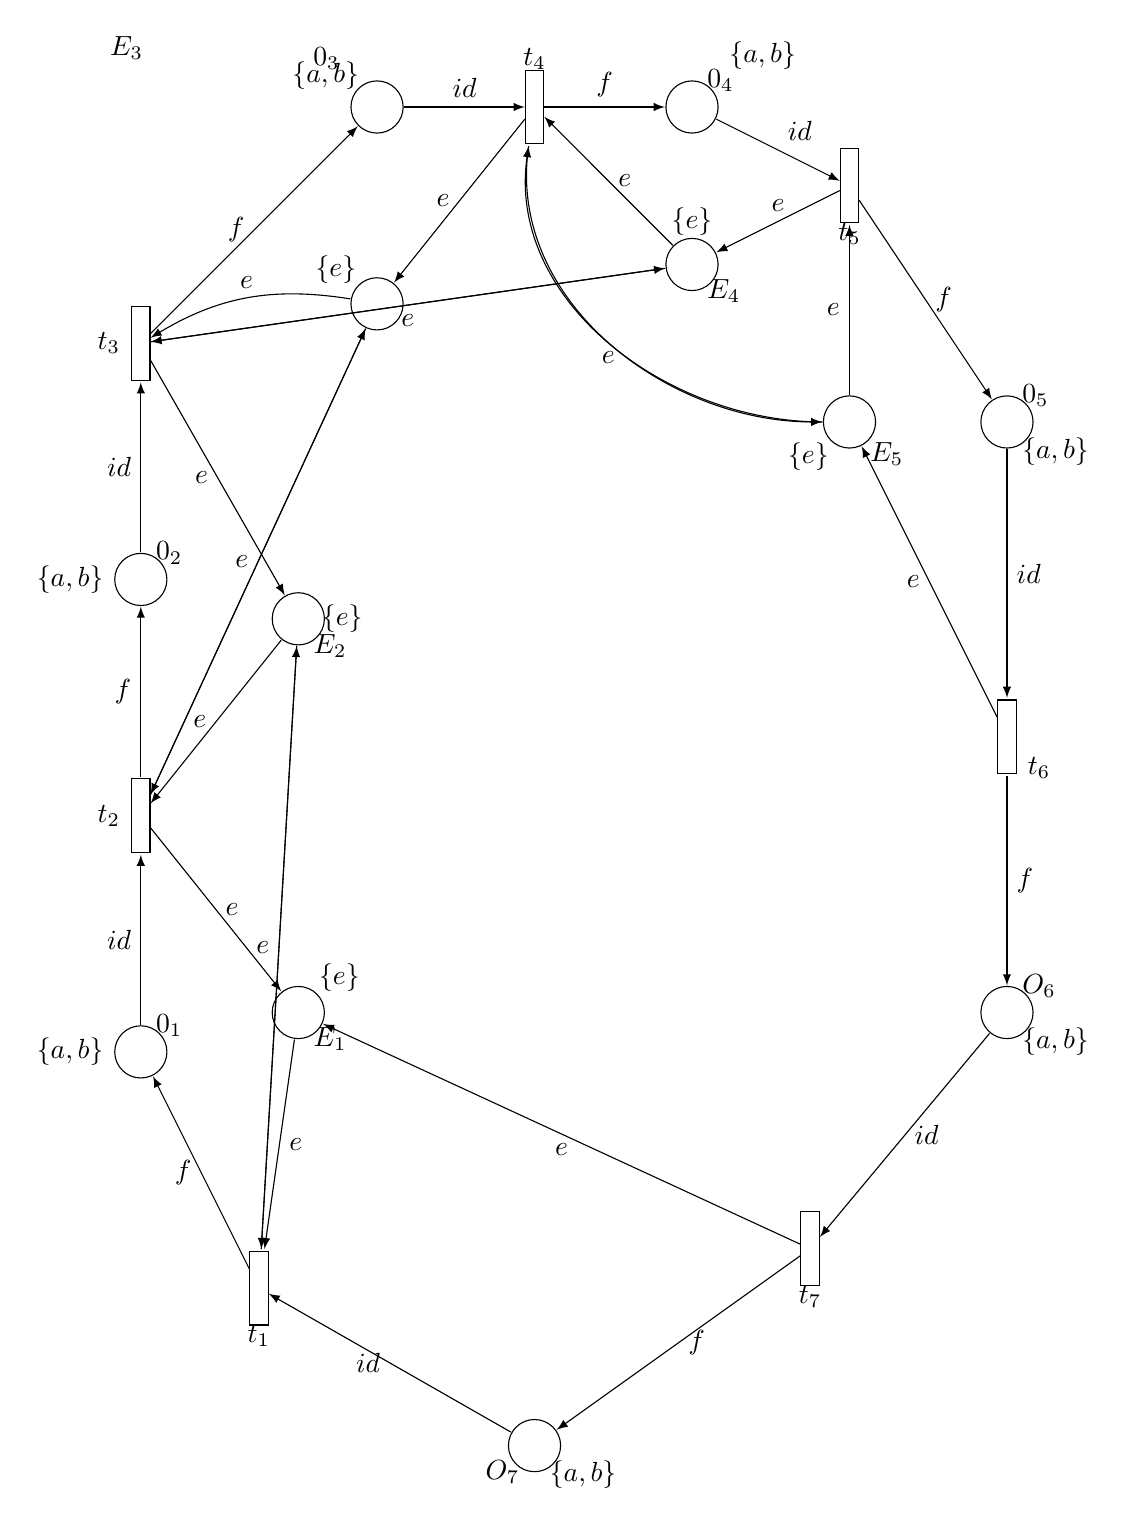
\begin{tikzpicture}

    % Liste des places
    \draw (0,-8) node[below left = 2pt] {$O_7$};
    \draw (0,-8) node[below right = 2pt] {$\{a,b\}$};
    \node[draw,circle,scale=2] (o7) at (0, -8) {};
    \draw (6,-2.5) node[above right = 2pt] {$O_6$};
    \draw (6,-2.5) node[below right = 2pt] {$\{a,b\}$};
    \node[draw,circle,scale=2] (o6) at (6, -2.5) {};
    \draw (6,5) node[above right = 2pt] {$0_5$};
    \draw (6,5) node[below right = 2pt] {$\{a,b\}$};
    \node[draw,circle,scale=2] (o5) at (6, 5) {};
    \draw (2,9) node[above right = 2pt] {$0_4$};
    \draw (2,9) node[above right = 10pt] {$\{a,b\}$};
    \node[draw,circle,scale=2] (o4) at (2, 9) {};
    \draw (-2,9) node[above left = 10pt] {$0_3$};
    \draw (-2,9) node[above left = 3pt] {$\{a,b\}$};
    \node[draw,circle,scale=2] (o3) at (-2, 9) {};
    \draw (-5,3) node[above right = 2pt] {$0_2$};
    \draw (-5,3) node[left = 10pt] {$\{a,b\}$};
    \node[draw,circle,scale=2] (o2) at (-5, 3) {};
    \draw (-5,-3) node[above right = 2pt] {$0_1$};
     \draw (-5,-3) node[left = 10pt] {$\{a,b\}$};
    \node[draw,circle,scale=2] (o1) at (-5, -3) {};
    \draw (-3,-2.5) node[below right = 2pt] {$E_1$};
    \draw (-3,-2.5) node[above right = 4pt] {$\{e\}$};
    \node[draw,circle,scale=2] (e1) at (-3, -2.5) {};
	\draw (-3,2.5) node[below right = 2pt] {$E_2$};
	\draw (-3,2.5) node[right = 5pt] {$\{e\}$};
    \node[draw,circle,scale=2] (e2) at (-3, 2.5) {};
    \draw (-2,6.5) node[below right = -100pt] {$E_3$};
    \draw (-2,6.5) node[above left = 4pt] {$\{e\}$};
    \node[draw,circle,scale=2] (e3) at (-2, 6.5) {};
    \draw (2, 7) node[below right = 2pt] {$E_4$};
    \draw (2,7) node[above = 7pt] {$\{e\}$};
    \node[draw,circle,scale=2] (e4) at (2, 7) {};
    \draw (4,5) node[below right = 4pt] {$E_5$};
    \draw (4,5) node[below left = 4pt] {$\{e\}$};
    \node[draw,circle,scale=2] (e5) at (4, 5) {};

    % Liste des transitions
    \draw (-3.5,-6) node[below = 10pt] {$t_1$};
    \node[draw,rectangle,yscale=4] (t1) at (-3.5, -6) {};
    \draw (-5,0) node[left = 4pt] {$t_2$};
    \node[draw,rectangle,yscale=4] (t2) at (-5, 0) {};
    \draw (-5,6) node[left = 4pt] {$t_3$};
    \node[draw,rectangle,yscale=4] (t3) at (-5, 6) {};
    \draw (0,9) node[above = 10pt] {$t_4$};
    \node[draw,rectangle,yscale=4] (t4) at (0, 9) {};
    \draw (4,8) node[below = 10pt] {$t_5$};
    \node[draw,rectangle,yscale=4] (t5) at (4, 8) {};
    \draw (6,1) node[below right = 4pt] {$t_6$};
    \node[draw,rectangle,yscale=4] (t6) at (6, 1) {};
    \draw (3.5,-5.5) node[below = 10pt] {$t_7$};
    \node[draw,rectangle,yscale=4] (t7) at (3.5, -5.5) {};

    % Liste des arcs
    \draw[->,>=latex] (o7) -- (t1) node[midway, left]{$id$};
    \draw[->,>=latex] (t1) -- (o1) node[midway, left]{$f$};
    \draw[->,>=latex] (o1) -- (t2) node[midway, left]{$id$};
    \draw[->,>=latex] (t2) -- (o2) node[midway, left]{$f$};
    \draw[->,>=latex] (o2) -- (t3) node[midway, left]{$id$};
    \draw[->,>=latex] (t3) -- (o3) node[midway, left]{$f$};
    \draw[->,>=latex] (o3) -- (t4) node[midway, above]{$id$};
    \draw[->,>=latex] (t4) -- (o4) node[midway, above]{$f$};
    \draw[->,>=latex] (o4) -- (t5) node[midway, above right]{$id$};
    \draw[->,>=latex] (t5) -- (o5) node[midway, right]{$f$};
    \draw[->,>=latex] (o5) -- (t6) node[midway, right]{$id$};
    \draw[->,>=latex] (t6) -- (o6) node[midway, right]{$f$};
    \draw[->,>=latex] (o6) -- (t7) node[midway, right]{$id$};
    \draw[->,>=latex] (t7) -- (o7) node[midway, right]{$f$};

    \draw[->,>=latex] (e1) -- (t1) node[midway, right]{$e$};
    \draw[->,>=latex] (t2) -- (e1) node[midway, right]{$e$};
    \draw[->,>=latex] (e2) -- (t1) node[midway, left]{$e$};
    \draw[->,>=latex] (t1) -- (e2);
    \draw[->,>=latex] (e3) -- (t2);
    \draw[->,>=latex] (t2) -- (e3) node[midway, left]{$e$}; 
    \draw[->,>=latex] (t3) -- (e2) node[midway, left]{$e$};
    \draw[->,>=latex] (e2) -- (t2) node[midway, left]{$e$};
    \draw[->,>=latex] (e3) to [bend right=20] node[midway, above]{$e$}(t3) ;
    \draw[->,>=latex] (t4) -- (e3) node[midway, left]{$e$};
    \draw[->,>=latex] (t3) -- (e4) node[midway, below]{$e$};
    \draw[->,>=latex] (e4) -- (t3);
    \draw[->,>=latex] (e4) -- (t4) node[midway, right]{$e$};
    \draw[->,>=latex] (t5) -- (e4) node[midway, above]{$e$};
    \draw[->,>=latex] (e5) to [out=-180, in=-100] node[midway, below]{$e$}(t4);
    \draw[->,>=latex] (t4) to [out=-100, in=-180] (e5);
    \draw[->,>=latex] (e5) -- (t5) node[midway, left]{$e$};
    \draw[->,>=latex] (t6) -- (e5) node[midway, left]{$e$};
    \draw[->,>=latex] (t7) -- (e1) node[midway, below]{$e$};
   


  \end{tikzpicture}
  \caption{Réseau de petri associé à 12.2} \label{fig:M1}
\end{figure}